\documentclass[tikz,border=10pt]{standalone}
\usepackage{tikz}
\usepackage{pgfplots}
\usetikzlibrary{shapes,arrows,positioning,fit,backgrounds,patterns}
\pgfplotsset{compat=1.16}

\begin{document}

% Figure 1: Enhanced System Architecture
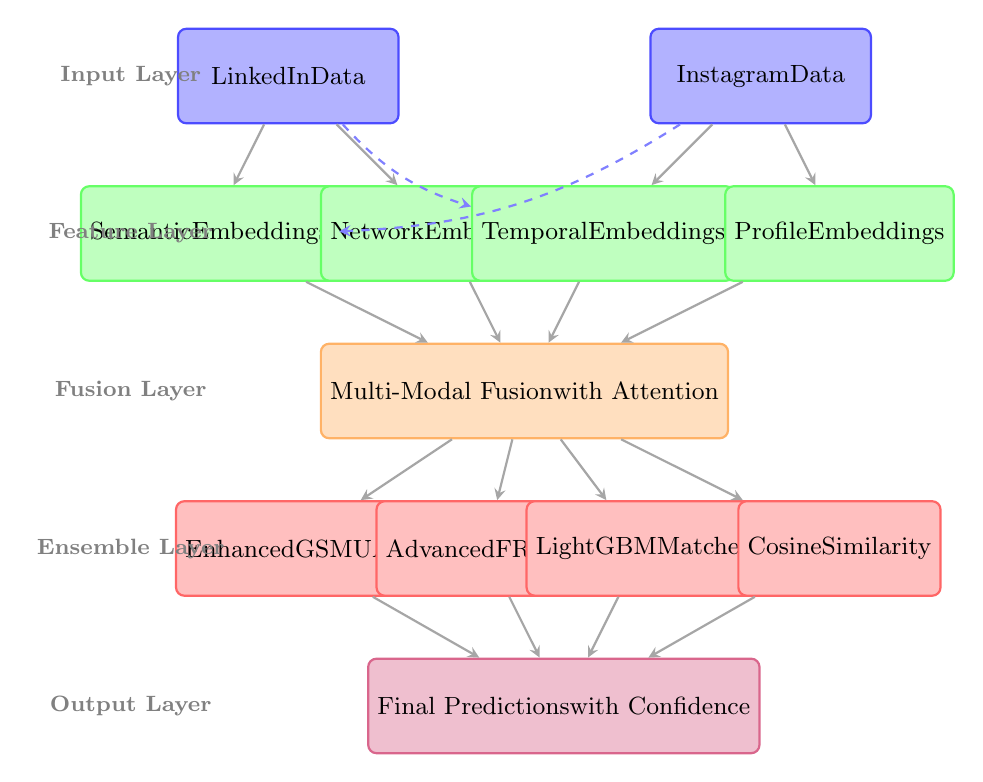
\begin{tikzpicture}[
    node distance=2cm,
    box/.style={rectangle, rounded corners=3pt, minimum width=2.8cm, minimum height=1.2cm,
                text centered, draw=black, line width=0.8pt, font=\small},
    inputbox/.style={box, fill=blue!30, draw=blue!70},
    processbox/.style={box, fill=green!25, draw=green!60},
    fusionbox/.style={box, fill=orange!25, draw=orange!60, minimum width=3.5cm},
    ensemblebox/.style={box, fill=red!25, draw=red!60, minimum width=2.5cm},
    outputbox/.style={box, fill=purple!25, draw=purple!60, minimum width=3cm},
    arrow/.style={thick,->,>=stealth, color=gray!70}
]

% Input Layer
\node[inputbox] (linkedin) at (0,7) {LinkedIn\\Data};
\node[inputbox] (instagram) at (6,7) {Instagram\\Data};

% Feature Extraction Layer
\node[processbox] (semantic) at (-1,5) {Semantic\\Embeddings};
\node[processbox] (network) at (2,5) {Network\\Embeddings};
\node[processbox] (temporal) at (4,5) {Temporal\\Embeddings};
\node[processbox] (profile) at (7,5) {Profile\\Embeddings};

% Fusion Layer
\node[fusionbox] (fusion) at (3,3) {Multi-Modal Fusion\\with Attention};

% Ensemble Layer
\node[ensemblebox] (gsmua) at (0,1) {Enhanced\\GSMUA};
\node[ensemblebox] (fruip) at (2.5,1) {Advanced\\FRUI-P};
\node[ensemblebox] (lgb) at (4.5,1) {LightGBM\\Matcher};
\node[ensemblebox] (cosine) at (7,1) {Cosine\\Similarity};

% Final Output
\node[outputbox] (output) at (3.5,-1) {Final Predictions\\with Confidence};

% Input to Feature Extraction Arrows
\draw[arrow] (linkedin) -- (semantic);
\draw[arrow] (linkedin) -- (network);
\draw[arrow] (instagram) -- (temporal);
\draw[arrow] (instagram) -- (profile);

% Cross-connections for multi-modal
\draw[arrow, dashed, color=blue!50] (linkedin) to[bend right=15] (temporal);
\draw[arrow, dashed, color=blue!50] (instagram) to[bend left=15] (semantic);

% Feature Extraction to Fusion
\draw[arrow] (semantic) -- (fusion);
\draw[arrow] (network) -- (fusion);
\draw[arrow] (temporal) -- (fusion);
\draw[arrow] (profile) -- (fusion);

% Fusion to Ensemble
\draw[arrow] (fusion) -- (gsmua);
\draw[arrow] (fusion) -- (fruip);
\draw[arrow] (fusion) -- (lgb);
\draw[arrow] (fusion) -- (cosine);

% Ensemble to Output
\draw[arrow] (gsmua) -- (output);
\draw[arrow] (fruip) -- (output);
\draw[arrow] (lgb) -- (output);
\draw[arrow] (cosine) -- (output);

% Layer labels
\node[font=\footnotesize, color=gray] at (-2,7) {\textbf{Input Layer}};
\node[font=\footnotesize, color=gray] at (-2,5) {\textbf{Feature Layer}};
\node[font=\footnotesize, color=gray] at (-2,3) {\textbf{Fusion Layer}};
\node[font=\footnotesize, color=gray] at (-2,1) {\textbf{Ensemble Layer}};
\node[font=\footnotesize, color=gray] at (-2,-1) {\textbf{Output Layer}};

\end{tikzpicture}

\newpage

% Figure 2: Multi-Modal Fusion Architecture
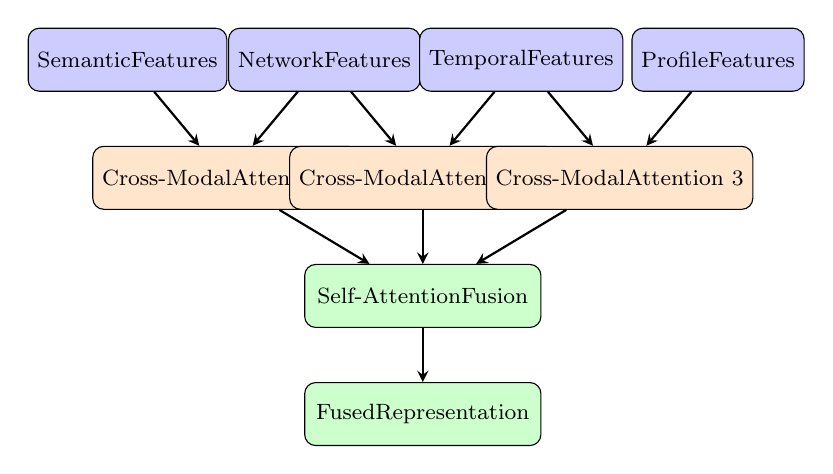
\begin{tikzpicture}[
    node distance=1cm,
    modalitybox/.style={rectangle, rounded corners, minimum width=2cm, minimum height=0.8cm, text centered, draw=black, fill=blue!20, font=\footnotesize},
    attentionbox/.style={rectangle, rounded corners, minimum width=2.5cm, minimum height=0.8cm, text centered, draw=black, fill=orange!20, font=\footnotesize},
    fusionbox/.style={rectangle, rounded corners, minimum width=3cm, minimum height=0.8cm, text centered, draw=black, fill=green!20, font=\footnotesize},
    arrow/.style={thick,->,>=stealth}
]

% Input modalities
\node[modalitybox] (sem) at (0,4) {Semantic\\Features};
\node[modalitybox] (net) at (2.5,4) {Network\\Features};
\node[modalitybox] (temp) at (5,4) {Temporal\\Features};
\node[modalitybox] (prof) at (7.5,4) {Profile\\Features};

% Cross-modal attention
\node[attentionbox] (crossatt1) at (1.25,2.5) {Cross-Modal\\Attention 1};
\node[attentionbox] (crossatt2) at (3.75,2.5) {Cross-Modal\\Attention 2};
\node[attentionbox] (crossatt3) at (6.25,2.5) {Cross-Modal\\Attention 3};

% Self-attention fusion
\node[fusionbox] (selfattn) at (3.75,1) {Self-Attention\\Fusion};

% Final output
\node[fusionbox] (output) at (3.75,-0.5) {Fused\\Representation};

% Arrows
\draw[arrow] (sem) -- (crossatt1);
\draw[arrow] (net) -- (crossatt1);
\draw[arrow] (net) -- (crossatt2);
\draw[arrow] (temp) -- (crossatt2);
\draw[arrow] (temp) -- (crossatt3);
\draw[arrow] (prof) -- (crossatt3);

\draw[arrow] (crossatt1) -- (selfattn);
\draw[arrow] (crossatt2) -- (selfattn);
\draw[arrow] (crossatt3) -- (selfattn);

\draw[arrow] (selfattn) -- (output);

\end{tikzpicture}

\newpage

% Figure 3: Performance Comparison Chart
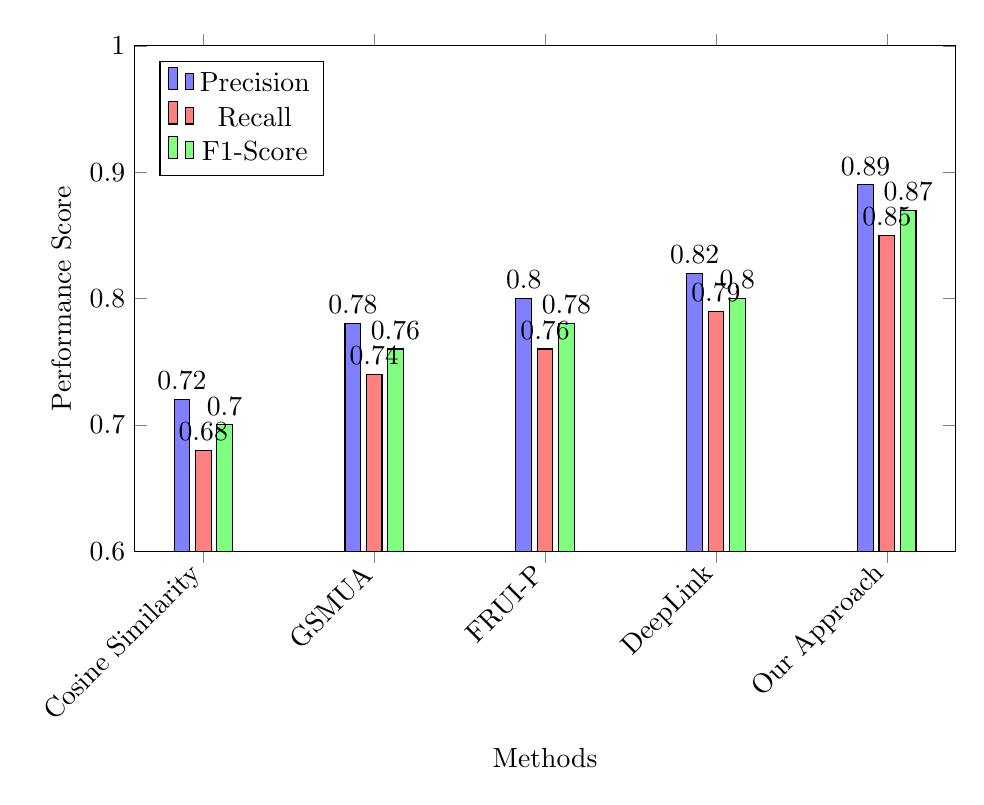
\begin{tikzpicture}
\begin{axis}[
    ybar,
    width=12cm,
    height=8cm,
    ylabel={Performance Score},
    xlabel={Methods},
    symbolic x coords={Cosine Similarity, GSMUA, FRUI-P, DeepLink, Our Approach},
    xtick=data,
    ymin=0.6,
    ymax=1.0,
    legend pos=north west,
    legend entries={Precision, Recall, F1-Score},
    bar width=0.2cm,
    nodes near coords,
    nodes near coords align={vertical},
    x tick label style={rotate=45,anchor=east},
]

% Precision
\addplot[fill=blue!50] coordinates {
    (Cosine Similarity,0.72)
    (GSMUA,0.78)
    (FRUI-P,0.80)
    (DeepLink,0.82)
    (Our Approach,0.89)
};

% Recall
\addplot[fill=red!50] coordinates {
    (Cosine Similarity,0.68)
    (GSMUA,0.74)
    (FRUI-P,0.76)
    (DeepLink,0.79)
    (Our Approach,0.85)
};

% F1-Score
\addplot[fill=green!50] coordinates {
    (Cosine Similarity,0.70)
    (GSMUA,0.76)
    (FRUI-P,0.78)
    (DeepLink,0.80)
    (Our Approach,0.87)
};

\end{axis}
\end{tikzpicture}

\newpage

% Figure 4: Ablation Study Results
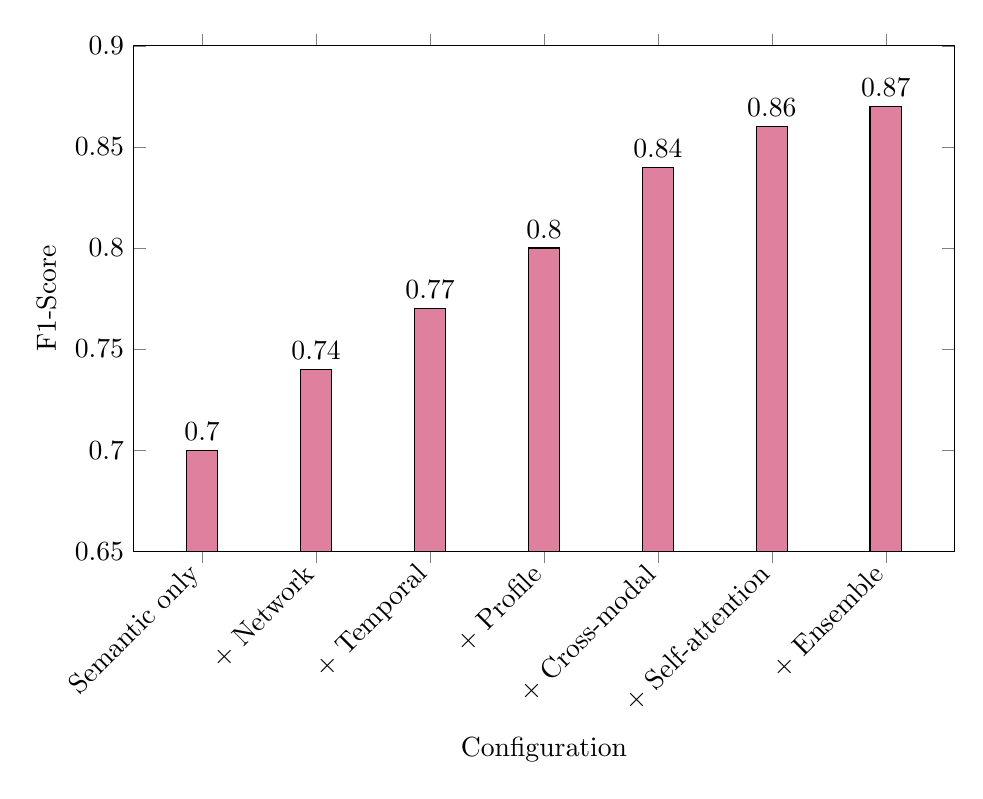
\begin{tikzpicture}
\begin{axis}[
    ybar,
    width=12cm,
    height=8cm,
    ylabel={F1-Score},
    xlabel={Configuration},
    symbolic x coords={Semantic only, + Network, + Temporal, + Profile, + Cross-modal, + Self-attention, + Ensemble},
    xtick=data,
    ymin=0.65,
    ymax=0.90,
    nodes near coords,
    nodes near coords align={vertical},
    x tick label style={rotate=45,anchor=east},
    bar width=0.4cm,
]

\addplot[fill=purple!50] coordinates {
    (Semantic only,0.70)
    (+ Network,0.74)
    (+ Temporal,0.77)
    (+ Profile,0.80)
    (+ Cross-modal,0.84)
    (+ Self-attention,0.86)
    (+ Ensemble,0.87)
};

\end{axis}
\end{tikzpicture}

\newpage

% Figure 5: Modality Contribution Analysis
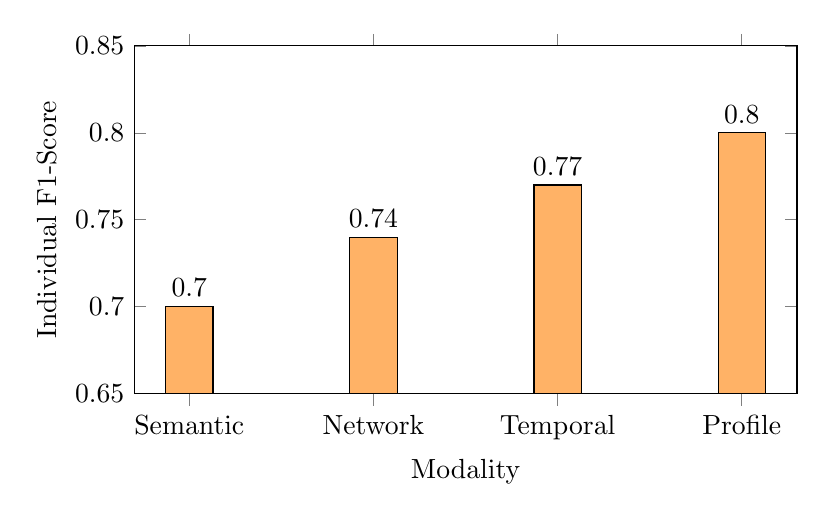
\begin{tikzpicture}
\begin{axis}[
    ybar,
    width=10cm,
    height=6cm,
    ylabel={Individual F1-Score},
    xlabel={Modality},
    symbolic x coords={Semantic, Network, Temporal, Profile},
    xtick=data,
    ymin=0.65,
    ymax=0.85,
    nodes near coords,
    nodes near coords align={vertical},
    bar width=0.6cm,
]

\addplot[fill=orange!60] coordinates {
    (Semantic,0.70)
    (Network,0.74)
    (Temporal,0.77)
    (Profile,0.80)
};

\end{axis}
\end{tikzpicture}

\newpage

% Figure 6: Ensemble Learning Architecture
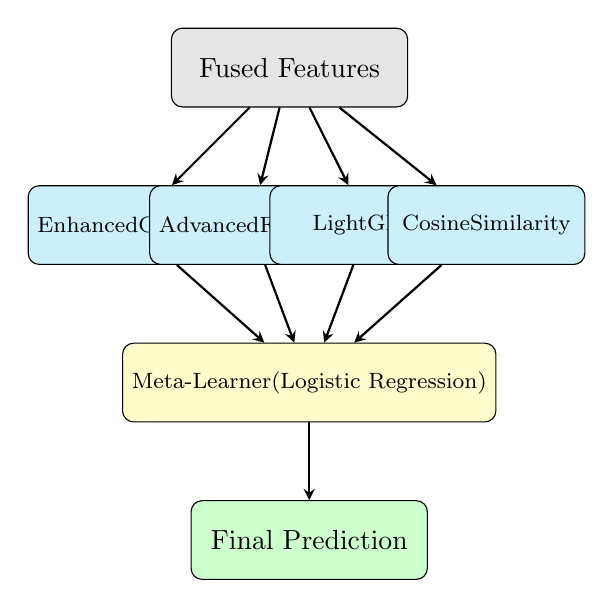
\begin{tikzpicture}[
    node distance=1.5cm,
    matcherbox/.style={rectangle, rounded corners, minimum width=2.5cm, minimum height=1cm, text centered, draw=black, fill=cyan!20, font=\footnotesize},
    metabox/.style={rectangle, rounded corners, minimum width=3cm, minimum height=1cm, text centered, draw=black, fill=yellow!20, font=\footnotesize},
    arrow/.style={thick,->,>=stealth}
]

% Input
\node[rectangle, rounded corners, minimum width=3cm, minimum height=1cm, text centered, draw=black, fill=gray!20] (input) at (2,6) {Fused Features};

% Base matchers
\node[matcherbox] (gsmua) at (0,4) {Enhanced\\GSMUA};
\node[matcherbox] (fruip) at (1.5,4) {Advanced\\FRUI-P};
\node[matcherbox] (lgb) at (3,4) {LightGBM};
\node[matcherbox] (cosine) at (4.5,4) {Cosine\\Similarity};

% Meta-learner
\node[metabox] (meta) at (2.25,2) {Meta-Learner\\(Logistic Regression)};

% Final output
\node[rectangle, rounded corners, minimum width=3cm, minimum height=1cm, text centered, draw=black, fill=green!20] (output) at (2.25,0) {Final Prediction};

% Arrows
\draw[arrow] (input) -- (gsmua);
\draw[arrow] (input) -- (fruip);
\draw[arrow] (input) -- (lgb);
\draw[arrow] (input) -- (cosine);

\draw[arrow] (gsmua) -- (meta);
\draw[arrow] (fruip) -- (meta);
\draw[arrow] (lgb) -- (meta);
\draw[arrow] (cosine) -- (meta);

\draw[arrow] (meta) -- (output);

\end{tikzpicture}

\end{document}
